\documentclass[1p]{elsarticle_modified}
%\bibliographystyle{elsarticle-num}

%\usepackage[colorlinks]{hyperref}
%\usepackage{abbrmath_seonhwa} %\Abb, \Ascr, \Acal ,\Abf, \Afrak
\usepackage{amsfonts}
\usepackage{amssymb}
\usepackage{amsmath}
\usepackage{amsthm}
\usepackage{scalefnt}
\usepackage{amsbsy}
\usepackage{kotex}
\usepackage{caption}
\usepackage{subfig}
\usepackage{color}
\usepackage{graphicx}
\usepackage{xcolor} %% white, black, red, green, blue, cyan, magenta, yellow
\usepackage{float}
\usepackage{setspace}
\usepackage{hyperref}

\usepackage{tikz}
\usetikzlibrary{arrows}

\usepackage{multirow}
\usepackage{array} % fixed length table
\usepackage{hhline}

%%%%%%%%%%%%%%%%%%%%%
\makeatletter
\renewcommand*\env@matrix[1][\arraystretch]{%
	\edef\arraystretch{#1}%
	\hskip -\arraycolsep
	\let\@ifnextchar\new@ifnextchar
	\array{*\c@MaxMatrixCols c}}
\makeatother %https://tex.stackexchange.com/questions/14071/how-can-i-increase-the-line-spacing-in-a-matrix
%%%%%%%%%%%%%%%

\usepackage[normalem]{ulem}

\newcommand{\msout}[1]{\ifmmode\text{\sout{\ensuremath{#1}}}\else\sout{#1}\fi}
%SOURCE: \msout is \stkout macro in https://tex.stackexchange.com/questions/20609/strikeout-in-math-mode

\newcommand{\cancel}[1]{
	\ifmmode
	{\color{red}\msout{#1}}
	\else
	{\color{red}\sout{#1}}
	\fi
}

\newcommand{\add}[1]{
	{\color{blue}\uwave{#1}}
}

\newcommand{\replace}[2]{
	\ifmmode
	{\color{red}\msout{#1}}{\color{blue}\uwave{#2}}
	\else
	{\color{red}\sout{#1}}{\color{blue}\uwave{#2}}
	\fi
}

\newcommand{\Sol}{\mathcal{S}} %segment
\newcommand{\D}{D} %diagram
\newcommand{\A}{\mathcal{A}} %arc


%%%%%%%%%%%%%%%%%%%%%%%%%%%%%5 test

\def\sl{\operatorname{\textup{SL}}(2,\Cbb)}
\def\psl{\operatorname{\textup{PSL}}(2,\Cbb)}
\def\quan{\mkern 1mu \triangleright \mkern 1mu}

\theoremstyle{definition}
\newtheorem{thm}{Theorem}[section]
\newtheorem{prop}[thm]{Proposition}
\newtheorem{lem}[thm]{Lemma}
\newtheorem{ques}[thm]{Question}
\newtheorem{cor}[thm]{Corollary}
\newtheorem{defn}[thm]{Definition}
\newtheorem{exam}[thm]{Example}
\newtheorem{rmk}[thm]{Remark}
\newtheorem{alg}[thm]{Algorithm}

\newcommand{\I}{\sqrt{-1}}
\begin{document}

%\begin{frontmatter}
%
%\title{Boundary parabolic representations of knots up to 8 crossings}
%
%%% Group authors per affiliation:
%\author{Yunhi Cho} 
%\address{Department of Mathematics, University of Seoul, Seoul, Korea}
%\ead{yhcho@uos.ac.kr}
%
%
%\author{Seonhwa Kim} %\fnref{s_kim}}
%\address{Center for Geometry and Physics, Institute for Basic Science, Pohang, 37673, Korea}
%\ead{ryeona17@ibs.re.kr}
%
%\author{Hyuk Kim}
%\address{Department of Mathematical Sciences, Seoul National University, Seoul 08826, Korea}
%\ead{hyukkim@snu.ac.kr}
%
%\author{Seokbeom Yoon}
%\address{Department of Mathematical Sciences, Seoul National University, Seoul, 08826,  Korea}
%\ead{sbyoon15@snu.ac.kr}
%
%\begin{abstract}
%We find all boundary parabolic representation of knots up to 8 crossings.
%
%\end{abstract}
%\begin{keyword}
%    \MSC[2010] 57M25 
%\end{keyword}
%
%\end{frontmatter}

%\linenumbers
%\tableofcontents
%
\newcommand\colored[1]{\textcolor{white}{\rule[-0.35ex]{0.8em}{1.4ex}}\kern-0.8em\color{red} #1}%
%\newcommand\colored[1]{\textcolor{white}{ #1}\kern-2.17ex	\textcolor{white}{ #1}\kern-1.81ex	\textcolor{white}{ #1}\kern-2.15ex\color{red}#1	}

{\Large $\underline{12a_{0437}~(K12a_{0437})}$}

\setlength{\tabcolsep}{10pt}
\renewcommand{\arraystretch}{1.6}
\vspace{1cm}\begin{tabular}{m{100pt}>{\centering\arraybackslash}m{274pt}}
\multirow{5}{120pt}{
	\centering
	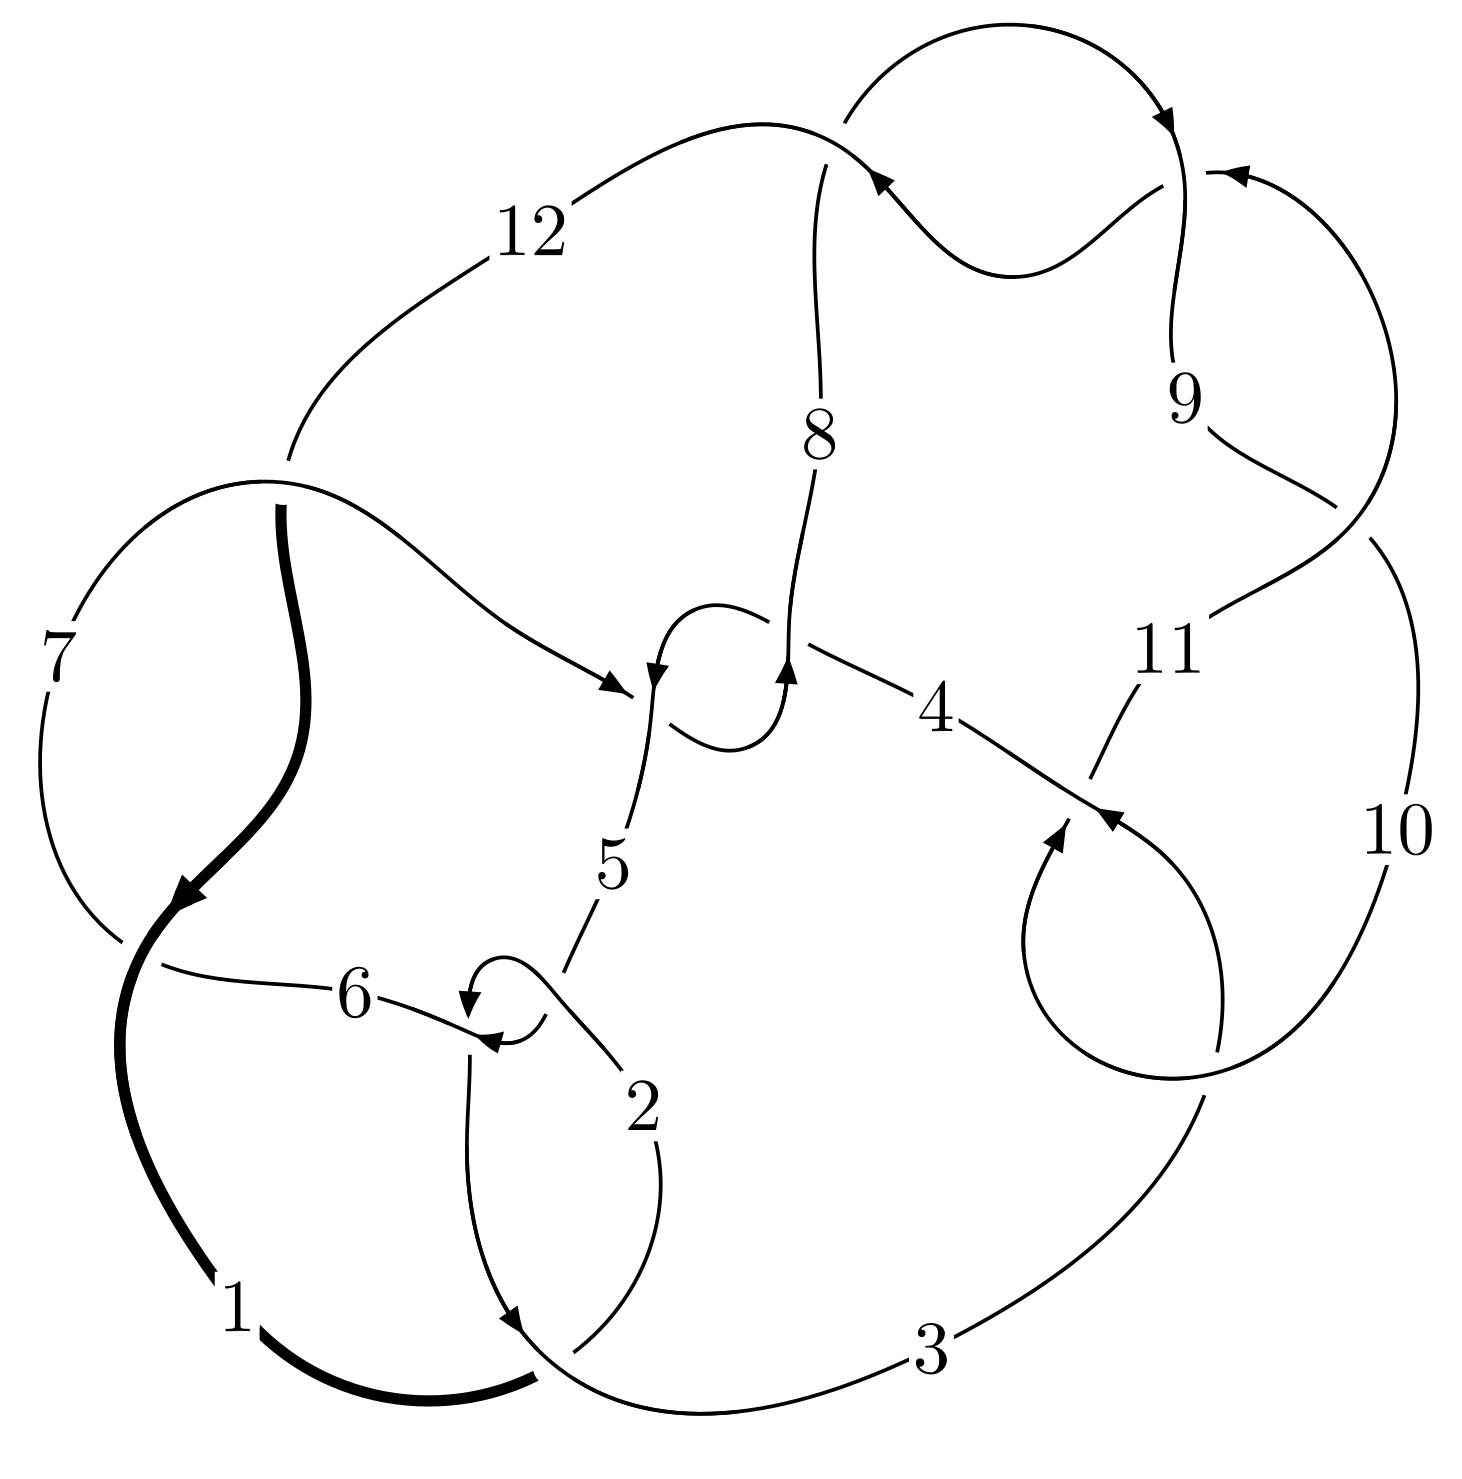
\includegraphics[width=112pt]{../../../GIT/diagram.site/Diagrams/png/1238_12a_0437.png}\\
\ \ \ A knot diagram\footnotemark}&
\allowdisplaybreaks
\textbf{Linearized knot diagam} \\
\cline{2-2}
 &
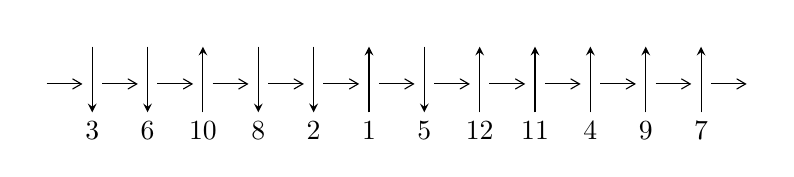
\begin{tikzpicture}[x=20pt, y=17pt]
	% nodes
	\node (C0) at (0, 0) {};
	\node (C1) at (1, 0) {};
	\node (C1U) at (1, +1) {};
	\node (C1D) at (1, -1) {3};

	\node (C2) at (2, 0) {};
	\node (C2U) at (2, +1) {};
	\node (C2D) at (2, -1) {6};

	\node (C3) at (3, 0) {};
	\node (C3U) at (3, +1) {};
	\node (C3D) at (3, -1) {10};

	\node (C4) at (4, 0) {};
	\node (C4U) at (4, +1) {};
	\node (C4D) at (4, -1) {8};

	\node (C5) at (5, 0) {};
	\node (C5U) at (5, +1) {};
	\node (C5D) at (5, -1) {2};

	\node (C6) at (6, 0) {};
	\node (C6U) at (6, +1) {};
	\node (C6D) at (6, -1) {1};

	\node (C7) at (7, 0) {};
	\node (C7U) at (7, +1) {};
	\node (C7D) at (7, -1) {5};

	\node (C8) at (8, 0) {};
	\node (C8U) at (8, +1) {};
	\node (C8D) at (8, -1) {12};

	\node (C9) at (9, 0) {};
	\node (C9U) at (9, +1) {};
	\node (C9D) at (9, -1) {11};

	\node (C10) at (10, 0) {};
	\node (C10U) at (10, +1) {};
	\node (C10D) at (10, -1) {4};

	\node (C11) at (11, 0) {};
	\node (C11U) at (11, +1) {};
	\node (C11D) at (11, -1) {9};

	\node (C12) at (12, 0) {};
	\node (C12U) at (12, +1) {};
	\node (C12D) at (12, -1) {7};
	\node (C13) at (13, 0) {};

	% arrows
	\draw[->,>={angle 60}]
	(C0) edge (C1) (C1) edge (C2) (C2) edge (C3) (C3) edge (C4) (C4) edge (C5) (C5) edge (C6) (C6) edge (C7) (C7) edge (C8) (C8) edge (C9) (C9) edge (C10) (C10) edge (C11) (C11) edge (C12) (C12) edge (C13) ;	\draw[->,>=stealth]
	(C1U) edge (C1D) (C2U) edge (C2D) (C3D) edge (C3U) (C4U) edge (C4D) (C5U) edge (C5D) (C6D) edge (C6U) (C7U) edge (C7D) (C8D) edge (C8U) (C9D) edge (C9U) (C10D) edge (C10U) (C11D) edge (C11U) (C12D) edge (C12U) ;
	\end{tikzpicture} \\
\hhline{~~} \\& 
\textbf{Solving Sequence} \\ \cline{2-2} 
 &
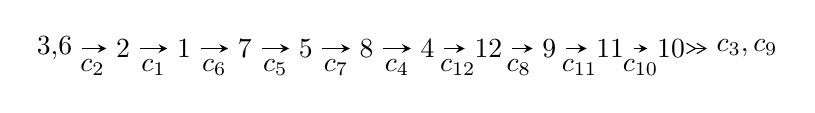
\begin{tikzpicture}[x=22pt, y=7pt]
	% node
	\node (A0) at (-1/8, 0) {3,6};
	\node (A1) at (1, 0) {2};
	\node (A2) at (2, 0) {1};
	\node (A3) at (3, 0) {7};
	\node (A4) at (4, 0) {5};
	\node (A5) at (5, 0) {8};
	\node (A6) at (6, 0) {4};
	\node (A7) at (7, 0) {12};
	\node (A8) at (8, 0) {9};
	\node (A9) at (9, 0) {11};
	\node (A10) at (10, 0) {10};
	\node (C1) at (1/2, -1) {$c_{2}$};
	\node (C2) at (3/2, -1) {$c_{1}$};
	\node (C3) at (5/2, -1) {$c_{6}$};
	\node (C4) at (7/2, -1) {$c_{5}$};
	\node (C5) at (9/2, -1) {$c_{7}$};
	\node (C6) at (11/2, -1) {$c_{4}$};
	\node (C7) at (13/2, -1) {$c_{12}$};
	\node (C8) at (15/2, -1) {$c_{8}$};
	\node (C9) at (17/2, -1) {$c_{11}$};
	\node (C10) at (19/2, -1) {$c_{10}$};
	\node (A11) at (45/4, 0) {$c_{3},c_{9}$};

	% edge
	\draw[->,>=stealth]	
	(A0) edge (A1) (A1) edge (A2) (A2) edge (A3) (A3) edge (A4) (A4) edge (A5) (A5) edge (A6) (A6) edge (A7) (A7) edge (A8) (A8) edge (A9) (A9) edge (A10) ;
	\draw[->>,>={angle 60}]	
	(A10) edge (A11);
\end{tikzpicture} \\ 

\end{tabular} \\

\footnotetext{
The image of knot diagram is generated by the software ``\textbf{Draw programme}" developed by Andrew Bartholomew(\url{http://www.layer8.co.uk/maths/draw/index.htm\#Running-draw}), where we modified some parts for our purpose(\url{https://github.com/CATsTAILs/LinksPainter}).
}\phantom \\ \newline 
\centering \textbf{Ideals for irreducible components\footnotemark of $X_{\text{par}}$} 
 
\begin{align*}
I^u_{1}&=\langle 
u^{74}- u^{73}+\cdots+u+1\rangle \\
\\
\end{align*}
\raggedright * 1 irreducible components of $\dim_{\mathbb{C}}=0$, with total 74 representations.\\
\footnotetext{All coefficients of polynomials are rational numbers. But the coefficients are sometimes approximated in decimal forms when there is not enough margin.}
\newpage
\renewcommand{\arraystretch}{1}
\centering \section*{I. $I^u_{1}= \langle u^{74}- u^{73}+\cdots+u+1 \rangle$}
\flushleft \textbf{(i) Arc colorings}\\
\begin{tabular}{m{7pt} m{180pt} m{7pt} m{180pt} }
\flushright $a_{3}=$&$\begin{pmatrix}1\\0\end{pmatrix}$ \\
\flushright $a_{6}=$&$\begin{pmatrix}0\\u\end{pmatrix}$ \\
\flushright $a_{2}=$&$\begin{pmatrix}1\\- u^2\end{pmatrix}$ \\
\flushright $a_{1}=$&$\begin{pmatrix}- u^2+1\\- u^2\end{pmatrix}$ \\
\flushright $a_{7}=$&$\begin{pmatrix}u^5-2 u^3+u\\u^5- u^3+u\end{pmatrix}$ \\
\flushright $a_{5}=$&$\begin{pmatrix}u\\- u^3+u\end{pmatrix}$ \\
\flushright $a_{8}=$&$\begin{pmatrix}- u^9+2 u^7- u^5-2 u^3+u\\u^{11}-3 u^9+4 u^7- u^5- u^3+u\end{pmatrix}$ \\
\flushright $a_{4}=$&$\begin{pmatrix}u^{17}-4 u^{15}+7 u^{13}-4 u^{11}-3 u^9+6 u^7-2 u^5+u\\- u^{19}+5 u^{17}-12 u^{15}+15 u^{13}-9 u^{11}- u^9+4 u^7-2 u^5- u^3+u\end{pmatrix}$ \\
\flushright $a_{12}=$&$\begin{pmatrix}- u^8+3 u^6-3 u^4+1\\- u^8+2 u^6-2 u^4\end{pmatrix}$ \\
\flushright $a_{9}=$&$\begin{pmatrix}u^{27}-8 u^{25}+\cdots-3 u^3+2 u\\u^{27}-7 u^{25}+\cdots- u^3+u\end{pmatrix}$ \\
\flushright $a_{11}=$&$\begin{pmatrix}- u^{46}+13 u^{44}+\cdots+2 u^2+1\\- u^{46}+12 u^{44}+\cdots-4 u^4+u^2\end{pmatrix}$ \\
\flushright $a_{10}=$&$\begin{pmatrix}- u^{65}+18 u^{63}+\cdots+2 u^3-3 u\\- u^{65}+17 u^{63}+\cdots+8 u^5- u\end{pmatrix}$\\&\end{tabular}
\flushleft \textbf{(ii) Obstruction class $= -1$}\\~\\
\flushleft \textbf{(iii) Cusp Shapes $= 4 u^{73}-80 u^{71}+\cdots-12 u+2$}\\~\\
\newpage\renewcommand{\arraystretch}{1}
\flushleft \textbf{(iv) u-Polynomials at the component}\newline \\
\begin{tabular}{m{50pt}|m{274pt}}
Crossings & \hspace{64pt}u-Polynomials at each crossing \\
\hline $$\begin{aligned}c_{1}\end{aligned}$$&$\begin{aligned}
&u^{74}+39 u^{73}+\cdots+3 u+1
\end{aligned}$\\
\hline $$\begin{aligned}c_{2},c_{5}\end{aligned}$$&$\begin{aligned}
&u^{74}+u^{73}+\cdots- u+1
\end{aligned}$\\
\hline $$\begin{aligned}c_{3},c_{10}\end{aligned}$$&$\begin{aligned}
&u^{74}+u^{73}+\cdots+u+1
\end{aligned}$\\
\hline $$\begin{aligned}c_{4},c_{7}\end{aligned}$$&$\begin{aligned}
&u^{74}-7 u^{73}+\cdots-39 u+5
\end{aligned}$\\
\hline $$\begin{aligned}c_{6},c_{12}\end{aligned}$$&$\begin{aligned}
&u^{74}+3 u^{73}+\cdots+91 u+39
\end{aligned}$\\
\hline $$\begin{aligned}c_{8},c_{9},c_{11}\end{aligned}$$&$\begin{aligned}
&u^{74}-19 u^{73}+\cdots-3 u+1
\end{aligned}$\\
\hline
\end{tabular}\\~\\
\newpage\renewcommand{\arraystretch}{1}
\flushleft \textbf{(v) Riley Polynomials at the component}\newline \\
\begin{tabular}{m{50pt}|m{274pt}}
Crossings & \hspace{64pt}Riley Polynomials at each crossing \\
\hline $$\begin{aligned}c_{1}\end{aligned}$$&$\begin{aligned}
&y^{74}-7 y^{73}+\cdots-3 y+1
\end{aligned}$\\
\hline $$\begin{aligned}c_{2},c_{5}\end{aligned}$$&$\begin{aligned}
&y^{74}-39 y^{73}+\cdots-3 y+1
\end{aligned}$\\
\hline $$\begin{aligned}c_{3},c_{10}\end{aligned}$$&$\begin{aligned}
&y^{74}-19 y^{73}+\cdots-3 y+1
\end{aligned}$\\
\hline $$\begin{aligned}c_{4},c_{7}\end{aligned}$$&$\begin{aligned}
&y^{74}+37 y^{73}+\cdots+2209 y+25
\end{aligned}$\\
\hline $$\begin{aligned}c_{6},c_{12}\end{aligned}$$&$\begin{aligned}
&y^{74}+53 y^{73}+\cdots+25961 y+1521
\end{aligned}$\\
\hline $$\begin{aligned}c_{8},c_{9},c_{11}\end{aligned}$$&$\begin{aligned}
&y^{74}+73 y^{73}+\cdots+5 y+1
\end{aligned}$\\
\hline
\end{tabular}\\~\\
\newpage\flushleft \textbf{(vi) Complex Volumes and Cusp Shapes}
$$\begin{array}{c|c|c}  
\text{Solutions to }I^u_{1}& \I (\text{vol} + \sqrt{-1}CS) & \text{Cusp shape}\\
 \hline 
\begin{aligned}
u &= -0.835681 + 0.560605 I\end{aligned}
 & -2.03574 + 3.50542 I & \phantom{-}2.00000 - 4.07643 I \\ \hline\begin{aligned}
u &= -0.835681 - 0.560605 I\end{aligned}
 & -2.03574 - 3.50542 I & \phantom{-}2.00000 + 4.07643 I \\ \hline\begin{aligned}
u &= \phantom{-}0.832665 + 0.571463 I\end{aligned}
 & -1.51570 - 9.58110 I & \phantom{-}2.00000 + 8.95690 I \\ \hline\begin{aligned}
u &= \phantom{-}0.832665 - 0.571463 I\end{aligned}
 & -1.51570 + 9.58110 I & \phantom{-}2.00000 - 8.95690 I \\ \hline\begin{aligned}
u &= \phantom{-}0.791742 + 0.569661 I\end{aligned}
 & \phantom{-}5.17088 - 5.15812 I & \phantom{-}8.32835 + 7.79457 I \\ \hline\begin{aligned}
u &= \phantom{-}0.791742 - 0.569661 I\end{aligned}
 & \phantom{-}5.17088 + 5.15812 I & \phantom{-}8.32835 - 7.79457 I \\ \hline\begin{aligned}
u &= \phantom{-}1.028500 + 0.160985 I\end{aligned}
 & -6.85388 + 0.05460 I & -5.85707 + 0. I\phantom{ +0.000000I} \\ \hline\begin{aligned}
u &= \phantom{-}1.028500 - 0.160985 I\end{aligned}
 & -6.85388 - 0.05460 I & -5.85707 + 0. I\phantom{ +0.000000I} \\ \hline\begin{aligned}
u &= -1.038800 + 0.183643 I\end{aligned}
 & -6.59018 + 6.05194 I & \phantom{-0.000000 } 0 \\ \hline\begin{aligned}
u &= -1.038800 - 0.183643 I\end{aligned}
 & -6.59018 - 6.05194 I & \phantom{-0.000000 } 0 \\ \hline\begin{aligned}
u &= -0.771164 + 0.538007 I\end{aligned}
 & \phantom{-}2.30346 + 2.17439 I & \phantom{-}2.29501 - 3.84413 I \\ \hline\begin{aligned}
u &= -0.771164 - 0.538007 I\end{aligned}
 & \phantom{-}2.30346 - 2.17439 I & \phantom{-}2.29501 + 3.84413 I \\ \hline\begin{aligned}
u &= \phantom{-}0.745955 + 0.571289 I\end{aligned}
 & \phantom{-}5.30206 + 0.62127 I & \phantom{-}9.02433 - 0.60864 I \\ \hline\begin{aligned}
u &= \phantom{-}0.745955 - 0.571289 I\end{aligned}
 & \phantom{-}5.30206 - 0.62127 I & \phantom{-}9.02433 + 0.60864 I \\ \hline\begin{aligned}
u &= -0.878223 + 0.286781 I\end{aligned}
 & -0.13660 + 3.04210 I & \phantom{-}1.28348 - 9.03887 I \\ \hline\begin{aligned}
u &= -0.878223 - 0.286781 I\end{aligned}
 & -0.13660 - 3.04210 I & \phantom{-}1.28348 + 9.03887 I \\ \hline\begin{aligned}
u &= \phantom{-}0.694463 + 0.581556 I\end{aligned}
 & -1.12248 + 5.01071 I & \phantom{-}3.66328 - 2.35709 I \\ \hline\begin{aligned}
u &= \phantom{-}0.694463 - 0.581556 I\end{aligned}
 & -1.12248 - 5.01071 I & \phantom{-}3.66328 + 2.35709 I \\ \hline\begin{aligned}
u &= -0.685413 + 0.567131 I\end{aligned}
 & -1.61031 + 0.99347 I & \phantom{-}2.79378 - 2.74942 I \\ \hline\begin{aligned}
u &= -0.685413 - 0.567131 I\end{aligned}
 & -1.61031 - 0.99347 I & \phantom{-}2.79378 + 2.74942 I \\ \hline\begin{aligned}
u &= \phantom{-}0.847866 + 0.088742 I\end{aligned}
 & -1.39303 - 0.27331 I & -6.60583 + 0.30491 I \\ \hline\begin{aligned}
u &= \phantom{-}0.847866 - 0.088742 I\end{aligned}
 & -1.39303 + 0.27331 I & -6.60583 - 0.30491 I \\ \hline\begin{aligned}
u &= \phantom{-}0.173274 + 0.798587 I\end{aligned}
 & -4.67079 + 10.47000 I & \phantom{-}0.63032 - 6.91545 I \\ \hline\begin{aligned}
u &= \phantom{-}0.173274 - 0.798587 I\end{aligned}
 & -4.67079 - 10.47000 I & \phantom{-}0.63032 + 6.91545 I \\ \hline\begin{aligned}
u &= -1.125660 + 0.366050 I\end{aligned}
 & -0.67532 + 2.89635 I & \phantom{-0.000000 } 0 \\ \hline\begin{aligned}
u &= -1.125660 - 0.366050 I\end{aligned}
 & -0.67532 - 2.89635 I & \phantom{-0.000000 } 0 \\ \hline\begin{aligned}
u &= -0.166312 + 0.795857 I\end{aligned}
 & -5.18741 - 4.27377 I & -0.40124 + 2.07461 I \\ \hline\begin{aligned}
u &= -0.166312 - 0.795857 I\end{aligned}
 & -5.18741 + 4.27377 I & -0.40124 - 2.07461 I \\ \hline\begin{aligned}
u &= \phantom{-}0.188589 + 0.769066 I\end{aligned}
 & \phantom{-}2.46946 + 6.12626 I & \phantom{-}6.02496 - 6.71747 I \\ \hline\begin{aligned}
u &= \phantom{-}0.188589 - 0.769066 I\end{aligned}
 & \phantom{-}2.46946 - 6.12626 I & \phantom{-}6.02496 + 6.71747 I\\
 \hline 
 \end{array}$$\newpage$$\begin{array}{c|c|c}  
\text{Solutions to }I^u_{1}& \I (\text{vol} + \sqrt{-1}CS) & \text{Cusp shape}\\
 \hline 
\begin{aligned}
u &= -1.110190 + 0.478729 I\end{aligned}
 & -5.42714 + 6.46328 I & \phantom{-0.000000 } 0 \\ \hline\begin{aligned}
u &= -1.110190 - 0.478729 I\end{aligned}
 & -5.42714 - 6.46328 I & \phantom{-0.000000 } 0 \\ \hline\begin{aligned}
u &= -0.005571 + 0.786467 I\end{aligned}
 & -9.15015 - 3.13723 I & -3.27787 + 2.62981 I \\ \hline\begin{aligned}
u &= -0.005571 - 0.786467 I\end{aligned}
 & -9.15015 + 3.13723 I & -3.27787 - 2.62981 I \\ \hline\begin{aligned}
u &= -1.174870 + 0.351936 I\end{aligned}
 & -1.57203 - 2.51139 I & \phantom{-0.000000 } 0 \\ \hline\begin{aligned}
u &= -1.174870 - 0.351936 I\end{aligned}
 & -1.57203 + 2.51139 I & \phantom{-0.000000 } 0 \\ \hline\begin{aligned}
u &= \phantom{-}1.120020 + 0.499746 I\end{aligned}
 & -5.15715 - 0.75516 I & \phantom{-0.000000 } 0 \\ \hline\begin{aligned}
u &= \phantom{-}1.120020 - 0.499746 I\end{aligned}
 & -5.15715 + 0.75516 I & \phantom{-0.000000 } 0 \\ \hline\begin{aligned}
u &= \phantom{-}1.169010 + 0.376170 I\end{aligned}
 & -3.98603 - 0.84644 I & \phantom{-0.000000 } 0 \\ \hline\begin{aligned}
u &= \phantom{-}1.169010 - 0.376170 I\end{aligned}
 & -3.98603 + 0.84644 I & \phantom{-0.000000 } 0 \\ \hline\begin{aligned}
u &= -0.166580 + 0.745150 I\end{aligned}
 & -0.14116 - 2.82982 I & -0.06496 + 2.64345 I \\ \hline\begin{aligned}
u &= -0.166580 - 0.745150 I\end{aligned}
 & -0.14116 + 2.82982 I & -0.06496 - 2.64345 I \\ \hline\begin{aligned}
u &= \phantom{-}1.169510 + 0.425972 I\end{aligned}
 & -5.43464 - 2.14338 I & \phantom{-0.000000 } 0 \\ \hline\begin{aligned}
u &= \phantom{-}1.169510 - 0.425972 I\end{aligned}
 & -5.43464 + 2.14338 I & \phantom{-0.000000 } 0 \\ \hline\begin{aligned}
u &= \phantom{-}0.210100 + 0.723982 I\end{aligned}
 & \phantom{-}3.11981 + 0.43939 I & \phantom{-}8.03831 + 0.99678 I \\ \hline\begin{aligned}
u &= \phantom{-}0.210100 - 0.723982 I\end{aligned}
 & \phantom{-}3.11981 - 0.43939 I & \phantom{-}8.03831 - 0.99678 I \\ \hline\begin{aligned}
u &= -1.201560 + 0.355229 I\end{aligned}
 & -8.81870 - 6.66835 I & \phantom{-0.000000 } 0 \\ \hline\begin{aligned}
u &= -1.201560 - 0.355229 I\end{aligned}
 & -8.81870 + 6.66835 I & \phantom{-0.000000 } 0 \\ \hline\begin{aligned}
u &= \phantom{-}1.201080 + 0.360636 I\end{aligned}
 & -9.29736 + 0.44713 I & \phantom{-0.000000 } 0 \\ \hline\begin{aligned}
u &= \phantom{-}1.201080 - 0.360636 I\end{aligned}
 & -9.29736 - 0.44713 I & \phantom{-0.000000 } 0 \\ \hline\begin{aligned}
u &= -1.165630 + 0.467482 I\end{aligned}
 & -5.13613 + 6.19077 I & \phantom{-0.000000 } 0 \\ \hline\begin{aligned}
u &= -1.165630 - 0.467482 I\end{aligned}
 & -5.13613 - 6.19077 I & \phantom{-0.000000 } 0 \\ \hline\begin{aligned}
u &= \phantom{-}1.153100 + 0.513557 I\end{aligned}
 & \phantom{-}0.38073 - 5.11443 I & \phantom{-0.000000 } 0 \\ \hline\begin{aligned}
u &= \phantom{-}1.153100 - 0.513557 I\end{aligned}
 & \phantom{-}0.38073 + 5.11443 I & \phantom{-0.000000 } 0 \\ \hline\begin{aligned}
u &= -1.168850 + 0.508704 I\end{aligned}
 & -3.05084 + 7.51931 I & \phantom{-0.000000 } 0 \\ \hline\begin{aligned}
u &= -1.168850 - 0.508704 I\end{aligned}
 & -3.05084 - 7.51931 I & \phantom{-0.000000 } 0 \\ \hline\begin{aligned}
u &= \phantom{-}1.170470 + 0.520288 I\end{aligned}
 & -0.40431 - 10.92870 I & \phantom{-0.000000 } 0 \\ \hline\begin{aligned}
u &= \phantom{-}1.170470 - 0.520288 I\end{aligned}
 & -0.40431 + 10.92870 I & \phantom{-0.000000 } 0 \\ \hline\begin{aligned}
u &= \phantom{-}0.275029 + 0.663064 I\end{aligned}
 & -2.70930 - 3.72938 I & \phantom{-}2.81438 + 3.00373 I \\ \hline\begin{aligned}
u &= \phantom{-}0.275029 - 0.663064 I\end{aligned}
 & -2.70930 + 3.72938 I & \phantom{-}2.81438 - 3.00373 I\\
 \hline 
 \end{array}$$\newpage$$\begin{array}{c|c|c}  
\text{Solutions to }I^u_{1}& \I (\text{vol} + \sqrt{-1}CS) & \text{Cusp shape}\\
 \hline 
\begin{aligned}
u &= \phantom{-}1.204050 + 0.448056 I\end{aligned}
 & -12.69820 - 1.26903 I & \phantom{-0.000000 } 0 \\ \hline\begin{aligned}
u &= \phantom{-}1.204050 - 0.448056 I\end{aligned}
 & -12.69820 + 1.26903 I & \phantom{-0.000000 } 0 \\ \hline\begin{aligned}
u &= -1.203510 + 0.453057 I\end{aligned}
 & -12.6628 + 7.5767 I & \phantom{-0.000000 } 0 \\ \hline\begin{aligned}
u &= -1.203510 - 0.453057 I\end{aligned}
 & -12.6628 - 7.5767 I & \phantom{-0.000000 } 0 \\ \hline\begin{aligned}
u &= -1.184440 + 0.519711 I\end{aligned}
 & -8.18403 + 9.13195 I & \phantom{-0.000000 } 0 \\ \hline\begin{aligned}
u &= -1.184440 - 0.519711 I\end{aligned}
 & -8.18403 - 9.13195 I & \phantom{-0.000000 } 0 \\ \hline\begin{aligned}
u &= -0.054792 + 0.704044 I\end{aligned}
 & -2.00051 - 1.86805 I & -1.34178 + 4.37957 I \\ \hline\begin{aligned}
u &= -0.054792 - 0.704044 I\end{aligned}
 & -2.00051 + 1.86805 I & -1.34178 - 4.37957 I \\ \hline\begin{aligned}
u &= \phantom{-}1.183790 + 0.522761 I\end{aligned}
 & -7.6480 - 15.3506 I & \phantom{-0.000000 } 0 \\ \hline\begin{aligned}
u &= \phantom{-}1.183790 - 0.522761 I\end{aligned}
 & -7.6480 + 15.3506 I & \phantom{-0.000000 } 0 \\ \hline\begin{aligned}
u &= -0.281349 + 0.627967 I\end{aligned}
 & -3.03701 - 2.14947 I & \phantom{-}2.22194 + 2.48741 I \\ \hline\begin{aligned}
u &= -0.281349 - 0.627967 I\end{aligned}
 & -3.03701 + 2.14947 I & \phantom{-}2.22194 - 2.48741 I \\ \hline\begin{aligned}
u &= -0.440598 + 0.299753 I\end{aligned}
 & \phantom{-}1.125240 - 0.112962 I & \phantom{-}9.20316 + 0.37924 I \\ \hline\begin{aligned}
u &= -0.440598 - 0.299753 I\end{aligned}
 & \phantom{-}1.125240 + 0.112962 I & \phantom{-}9.20316 - 0.37924 I\\
 \hline 
 \end{array}$$\newpage
\newpage\renewcommand{\arraystretch}{1}
\centering \section*{ II. u-Polynomials}
\begin{tabular}{m{50pt}|m{274pt}}
Crossings & \hspace{64pt}u-Polynomials at each crossing \\
\hline $$\begin{aligned}c_{1}\end{aligned}$$&$\begin{aligned}
&u^{74}+39 u^{73}+\cdots+3 u+1
\end{aligned}$\\
\hline $$\begin{aligned}c_{2},c_{5}\end{aligned}$$&$\begin{aligned}
&u^{74}+u^{73}+\cdots- u+1
\end{aligned}$\\
\hline $$\begin{aligned}c_{3},c_{10}\end{aligned}$$&$\begin{aligned}
&u^{74}+u^{73}+\cdots+u+1
\end{aligned}$\\
\hline $$\begin{aligned}c_{4},c_{7}\end{aligned}$$&$\begin{aligned}
&u^{74}-7 u^{73}+\cdots-39 u+5
\end{aligned}$\\
\hline $$\begin{aligned}c_{6},c_{12}\end{aligned}$$&$\begin{aligned}
&u^{74}+3 u^{73}+\cdots+91 u+39
\end{aligned}$\\
\hline $$\begin{aligned}c_{8},c_{9},c_{11}\end{aligned}$$&$\begin{aligned}
&u^{74}-19 u^{73}+\cdots-3 u+1
\end{aligned}$\\
\hline
\end{tabular}\newpage\renewcommand{\arraystretch}{1}
\centering \section*{ III. Riley Polynomials}
\begin{tabular}{m{50pt}|m{274pt}}
Crossings & \hspace{64pt}Riley Polynomials at each crossing \\
\hline $$\begin{aligned}c_{1}\end{aligned}$$&$\begin{aligned}
&y^{74}-7 y^{73}+\cdots-3 y+1
\end{aligned}$\\
\hline $$\begin{aligned}c_{2},c_{5}\end{aligned}$$&$\begin{aligned}
&y^{74}-39 y^{73}+\cdots-3 y+1
\end{aligned}$\\
\hline $$\begin{aligned}c_{3},c_{10}\end{aligned}$$&$\begin{aligned}
&y^{74}-19 y^{73}+\cdots-3 y+1
\end{aligned}$\\
\hline $$\begin{aligned}c_{4},c_{7}\end{aligned}$$&$\begin{aligned}
&y^{74}+37 y^{73}+\cdots+2209 y+25
\end{aligned}$\\
\hline $$\begin{aligned}c_{6},c_{12}\end{aligned}$$&$\begin{aligned}
&y^{74}+53 y^{73}+\cdots+25961 y+1521
\end{aligned}$\\
\hline $$\begin{aligned}c_{8},c_{9},c_{11}\end{aligned}$$&$\begin{aligned}
&y^{74}+73 y^{73}+\cdots+5 y+1
\end{aligned}$\\
\hline
\end{tabular}
\vskip 2pc
\end{document}